\section{Gaia-X}
\label{sec:grundlagen:gaia-x}
Europas Plan für digitale Souveränität besteht aus der Cloud- sowie Datenselbstbestimmung.
Cloudsouveränität ist wichtig, um Services zu nutzen, die europäischen Regulierungen entsprechen \cite{Braud2021}.
Gaia-X ist hierfür die Initiative, einen freien Software Stack für Kontrolle, Governance und Erstellung gemeinsamer
Regeln und Richtlinien zu entwickeln \cite{Bonfiglio2021}. 
Dieser Stack soll auf allen bestehenden Cloudtechnologien anwendbar sein, um Transparenz, Souveränität und 
Interoperabilität bei Datenübermittlung und Dienstleistungen zu erreichen \cite{Bonfiglio2021}.

\subsection{Architektur}
\label{subsec:gaia-x:architektur}
\paragraph{Design Prinzipien}
Die Gaia-X Architektur beruht auf den folgenden Design Prinzipien:

\subparagraph{Föderationen}
Föderalisierte Systeme beschreiben autonome Einheiten, die durch eine spezifizierte Reihe von Normen,
Frameworks und Regeln verbunden sind \cite{GaiaXArchitecture2021}.
Das Prinzip soll mit einer minimalen Anzahl an Vorgaben die Interoperabilität und den Informationsaustausch
zwischen den einzelnen Einheiten der Föderation ermöglichen \cite{GaiaXArchitecture2021}. 
Dabei soll gleichzeitig das Höchstmaß an Autonomie gewährleistet werden \cite{GaiaXArchitecture2021}.
Durch Föderationen können Serviceanbieter ihre Infrastruktur auf vertrauenswürde Weise miteinander verbinden,
um ein verteiltes Cloud-Modell anzubieten \cite{Bonfiglio2021}.

\subparagraph{Dezentralisierung}
Mitglieder einer Föderation sollen selbstorganisiert, ohne zentrale Kontrolle, operieren.
Das Föderationsprinzip ermöglicht diese Selbstorganisation durch die Bereitstellung eines Netzwerks
zur Interaktion mit anderen Gaia-X Teilnehmern \cite{GaiaXArchitecture2021}.

\subparagraph{Offenheit}
Eine offene Architektur ermöglicht das einfache Hinzufügen, Aktualisieren und Ändern von Komponenten, sowie
Einblicke in alle Teile der Architektur und proprietäre Nutzung von Software.
Dadurch ist Gaia-X offen für zukünftige Innovationen und Standards und fortschreitende Technologie \cite{GaiaXArchitecture2021}.

\begin{figure}[h]
  \centering
  \makebox[\textwidth][c]{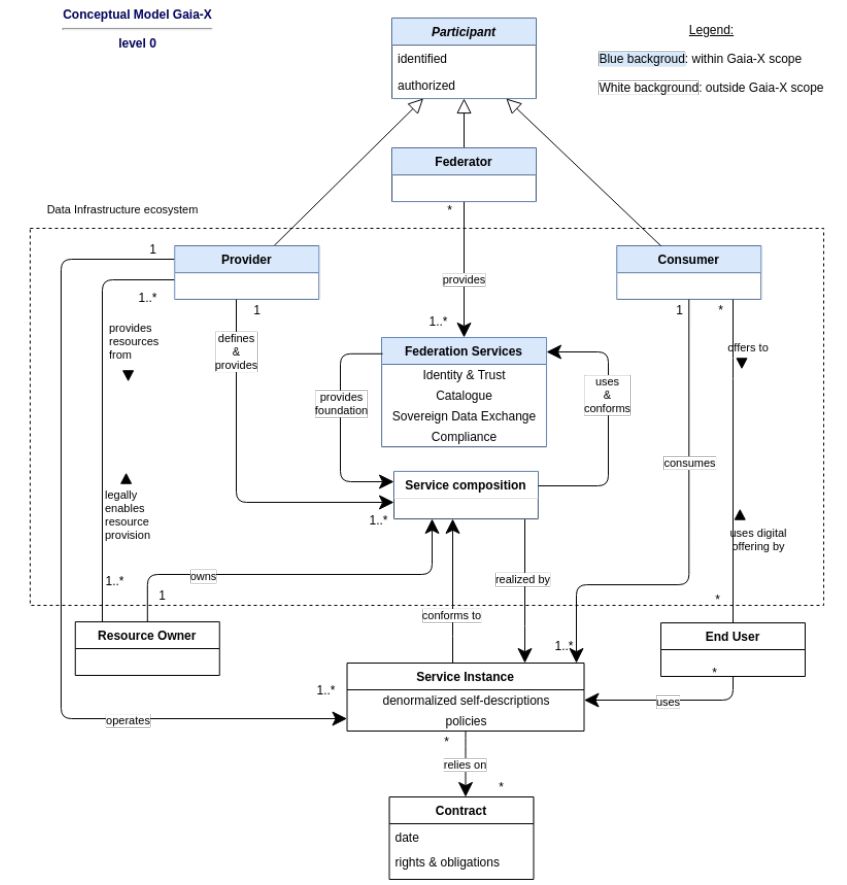
\includegraphics[width=1.25\textwidth]{gfx/chapters/2_grundlagen/gaia-x-architecture.png}}
  \caption{Konzeptuelles Modell der Gaia-X Architektur}
  \source{\cite{GaiaXArchitecture2021}}
  \label{fig:gaia-x-concept-architecture}
\end{figure}

\paragraph{Architekturkonzept}
In Abbildung \ref{fig:gaia-x-concept-architecture} wird das Architekturkonzept, sowie der Umfang von Gaia-X verdeutlich.
Die obere Hälfte des Modells zeigt die verschiedenen Akteure innerhalb von Gaia-X, während die
untere Hälfte den Umfang sowie das Zusammenspiel der Mitglieder außerhalb von Gaia-X darstellt \cite{GaiaXArchitecture2021}.

\subparagraph{Participants}
Participants sind Teilnehmer innerhalb von Gaia-X. 
Dabei können sie eine oder mehrere Rollen einehmen: Anbieter, Föderalist oder Konsument \cite{GaiaXArchitecture2021}.

\subparagraph{Anbieter}
Anbieter sind Teilnehmer, die Ressourcen im Gaia-X Ökosystem bereitstellen. Zudem stellt
ein Anbieter Services mit deren allgemeinen Geschäftsbedingungen und technischen Richtlinien bereit \cite{GaiaXArchitecture2021}.

\subparagraph{Föderalist}
Ein Föderalist ist für die Implementierung der Föderationsservices (siehe \ref{subsec:gaia-x:federationservices}) 
sowie für die Koordination der Teilnehmer innerhalb einer Föderation zuständig \cite{GXFS2021}.

\subparagraph{Konsument}
Konsumenten nutzen die von Providern bereitgestellten Services im Gaia-X Ökosystem, um digitale Angebote für Kunden zu ermöglichen \cite{GaiaXArchitecture2021}.

\subsection{Föderationsservices}
\label{subsec:gaia-x:federationservices}
Föderationsservices können als minimale technische Anforderungen zur Operativität einer Föderation angesehen werden \cite{GXFS2021}.
Dabei werden Services definiert, welche zur Erfüllung der Ziele von Gaia-X, Vertrauen und Interoperabilität
aufzubauen, sowie die Sicherstellung von Datensouveränität für Teilnehmer zu gewährleisten, beitragen \cite{GXFS2021}.
Zum Start des Gaia-X Projekts werden die folgenden vier Services definiert:

\paragraph{Identität und Vertrauen}
Teilnehmer einer Föderation nehmen diesen Service in Anspruch, um Authentifizierung und Autorisierung innerhalb der Föderation zu nutzen \cite{GXFS2021}.

\paragraph{Föderalisierter Katalog}
Der Katalog dient als zentrales 
Repository\footnote{Verzeichnis zur Speicherung und Verwaltung von digitalen Informationen} 
einer Föderation.
Er ermöglicht Teilnehmern das Finden von Informationen und Diensten anderer Föderationsteilnehmer durch Nutzung von
\emph{Self-Descriptions} (siehe \ref{sec:gaia-x-einbettung:gaia-x-katalog}) \cite{GXFS2021}.

\paragraph{Datensouveränität}
Dieser Service hilft Teilnehmern der Föderation die Kontrolle und Überblick über ihre Daten zu behalten.
Dabei werden Verfahren implementiert, um Transparenz und Kontrolle über Datennutzung zu definieren \cite{GXFS2021}.

\paragraph{Konformität}
Konformitätsservices ermöglichen die Überprüfung der gemeinsamen Services in einer Föderation auf Einhaltung
von Gaia-X Prinzipien, wie den Anspruch an gewisse Datensicherheit \cite{GXFS2021}.
